\section{Calibration}
\label{sec:calibration}

Two resource parameters were calibrated against the model's own generated
worlds rather than chosen by hand. Both calibrations are reproduced by
\texttt{experiments/e3-ice-structure.mjs}.

\subsection{Ice richness is banded}

Sampling every ice tile across eight generated polar worlds
($n = 4{,}187$) shows that richness is not continuous but falls into narrow
bands (Figure~\ref{fig:ice}, left). This follows directly from the derivation:
richness is an affine function of solar exposure, and exposure is the output of
a raycast over a quantised elevation field, so it takes a small number of
discrete values.

The practical consequence is that a richness threshold is only meaningful if it
falls between bands. A threshold inside a band selects everything or nothing.
This is worth stating because it is invisible from the parameter alone: a
richness requirement of $0.62$ looks like a mild constraint and is in fact,
at polar latitudes where the sampled range is $0.621$ to $0.896$, no
constraint at all on naturally occurring sites. It binds only on ground the
player has deliberately levelled out of a partially shadowed slope.

\subsection{The yield divisor}

A bore's output scales with a yield derived by dividing the ice within reach by
a reference constant and clamping the result to $[0.25, 1.5]$. Choosing that
divisor badly is not a matter of balance but of information: too small a value
pins sites against the upper clamp, and a saturated site absorbs the penalty
for crowding two bores onto one deposit without showing it.

Sampling the raw ice sum at every legal bore site across eight worlds
($n = 380$) gives a median of $9.31$ and a maximum of $15.85$. Sweeping the
divisor (Table~\ref{tab:sweep}, Figure~\ref{fig:ice} right) shows the obvious
choice of 8 --- which places the median site at unity --- pinning $19.5\%$ of
all legal sites against the ceiling. The chosen value of 12 is the smallest
divisor at which no site saturates, leaving the crowding penalty always
visible.

\begin{table}[htbp]
\centering
\caption{Yield divisor sweep over 380 legal bore sites from eight generated
polar worlds. The chosen value is the smallest at which no site is pinned
against the upper clamp.}
\label{tab:sweep}
\begin{tabular}{rrrr}
\toprule
divisor & median yield & 95th percentile & \% at ceiling \\
\midrule
 6 & 1.500 & 1.500 & 52.6 \\
 8 & 1.163 & 1.500 & 19.5 \\
10 & 0.931 & 1.379 &  0.8 \\
\textbf{12} & \textbf{0.775} & \textbf{1.149} & \textbf{0.0} \\
14 & 0.665 & 0.985 &  0.0 \\
16 & 0.582 & 0.862 &  0.0 \\
\bottomrule
\end{tabular}
\end{table}

\begin{figure}[htbp]
\centering
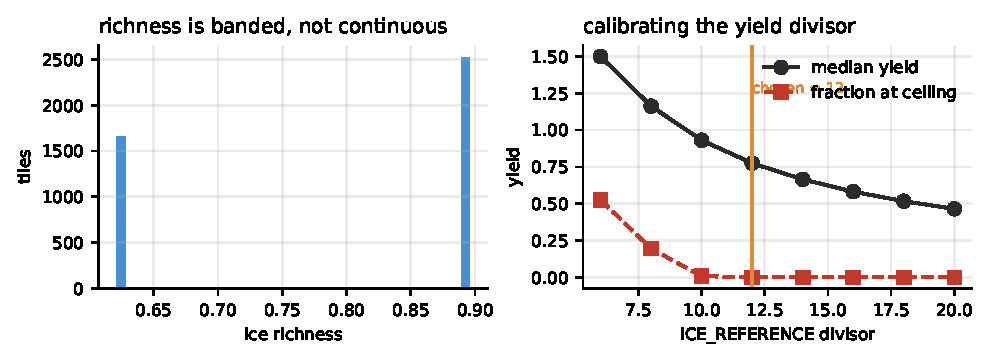
\includegraphics[width=\textwidth]{figures/ice-structure.pdf}
\caption{Left: ice richness across eight generated polar worlds, showing the
banding that follows from a quantised illumination model. Right: the yield
divisor sweep; the chosen value is the smallest at which no site saturates.}
\label{fig:ice}
\end{figure}
